\chapter{DIAC}
  \begin{wrapfigure}{R}{0.3\textwidth}
  \vspace{-1cm}
    \centering
    \resizebox{!}{\linewidth}{
    \begin{tikzpicture}
	\begin{pgfonlayer}{nodelayer}
		\node [style=none] (0) at (-1, 1.5) {};
		\node [style=none] (2) at (-1, 0.5) {};
		\node [style=none] (3) at (1, 0.5) {};
		\node [style=none] (4) at (-1, -0.5) {};
		\node [style=none] (5) at (1, -0.5) {};
		\node [style=none] (28) at (0, 1) {p};
		\node [style=none] (29) at (0, 0) {n};
		\node [style=none] (30) at (0, -1) {p};
		\node [style=none] (31) at (1, 2.5) {};
		\node [style=none] (32) at (0, 2.5) {};
		\node [style=none] (33) at (0, 1.5) {};
		\node [style=none] (34) at (-1, 2.5) {};
		\node [style=none] (35) at (1, 0.5) {};
		\node [style=none] (36) at (-1, -2.5) {};
		\node [style=none] (37) at (0, -2.5) {};
		\node [style=none] (38) at (0, -1.5) {};
		\node [style=none] (39) at (1, -2.5) {};
		\node [style=none] (40) at (1, -1.5) {};
		\node [style=none] (41) at (-0.5, 2) {n};
		\node [style=none] (42) at (0.5, -2) {n};
		\node [style=none] (43) at (-0.5, 2.5) {};
		\node [style=none] (44) at (-0.5, 2.75) {};
		\node [style=none] (45) at (0.5, 2.75) {};
		\node [style=none] (46) at (0.5, 2.5) {};
		\node [style=none] (47) at (-0.5, -2.5) {};
		\node [style=none] (48) at (0.5, -2.5) {};
		\node [style=none] (49) at (-0.5, -2.75) {};
		\node [style=none] (50) at (0.5, -2.75) {};
		\node [style=none] (51) at (0, 2.75) {};
		\node [style=none] (52) at (0, 3.25) {};
		\node [style=none] (53) at (0, 3.75) {$A_1$};
		\node [style=none] (54) at (0, -2.75) {};
		\node [style=none] (55) at (0, -3.25) {};
		\node [style=none] (56) at (0, -3.75) {$A_2$};
	\end{pgfonlayer}
	\begin{pgfonlayer}{edgelayer}
		\draw [style=fill2] (3.center) to (2.center);
		\draw [style=fill2] (2.center)
			 to (35.center)
			 to (31.center)
			 to (32.center)
			 to (33.center)
			 to (0.center)
			 to cycle;
		\draw [style=fill2] (5.center) to (4.center);
		\draw [style=fill3] (4.center)
			 to (5.center)
			 to (3.center)
			 to (2.center)
			 to cycle;
		\draw [style=fill2] (4.center)
			 to (36.center)
			 to (37.center)
			 to (38.center)
			 to (40.center)
			 to (5.center)
			 to cycle;
		\draw [style=fill3] (33.center)
			 to (32.center)
			 to (34.center)
			 to (0.center)
			 to cycle;
		\draw [style=fill3] (37.center)
			 to (39.center)
			 to (40.center)
			 to (38.center)
			 to cycle;
		\draw [style=fill4] (44.center)
			 to (45.center)
			 to (46.center)
			 to (43.center)
			 to cycle;
		\draw [style=fill4] (49.center)
			 to (50.center)
			 to (48.center)
			 to (47.center)
			 to cycle;
		\draw (51.center) to (52.center);
		\draw (54.center) to (55.center);
	\end{pgfonlayer}
\end{tikzpicture}

    }
    \caption{estructura interna del DIAC.}
    \label{fig:diac_si}
  \end{wrapfigure}
  Un DIAC es un dispositivo semiconductor de cuatro capas y dos terminales (tiristor) que conduce corriente en una u
  otra dirección cuando se activa. La construcción básica de un DIAC se muestran en la figura \ref{fig:scr_si}. Observe
  las dos terminales, designadas A1 y A2. Las capas superior e inferior contienen tanto materiales n como p. El lado
  derecho de la pila se considera como una estructura pnpn con las mismas características de un diodo de cuatro capas,
  mientras que el lado izquierdo es un diodo de cuatro capas invertido que tiene una estructura npnp.

  La conducción ocurre en un DIAC cuando se alcanza el voltaje de ruptura con una u otra polaridad a través de las dos
  terminales. Una vez que se presenta la ruptura, la corriente fluye en una dirección según la polaridad del voltaje a
  través de las terminales. El dispositivo se apaga cuando la corriente se reduce por debajo del valor de retención.

  \section{Reversibilidad del DIAC}
    Para esta actividad de laboratorio, se propuso variar la tensión de alimentación de 0 a 50V, en pasos de 5V, e ir
    midiendo la corriente que circula por el circuito. Una vez completada la prueba, se debe invertir la polaridad del
    circuito y realizar las mismas mediciones. El circuito implementado en el laboratorio se puede ver en la figura
    \ref{crkt:diac_lab}.

    \begin{figure}[!ht]
      \centering
      \begin{minipage}{0.5\textwidth}
        \centering
        \begin{tikzpicture}
	% Paths, nodes and wires:
	\draw (0, 3.5) to[empty bidirectionaldiode] (0, 1.75);
	\draw (0, 3.5) to[american resistor, l={$R_1$}] (0, 5.5);
	\draw (-0, 1.75) to[qiprobe, l={$I_A$}] (-0, -0);
	\draw (2, 3.5) to[qvprobe, l={$V_A$}] (2, -0);
	\draw (4, 5.5) to[qvprobe, l={$V$}] (4, -0);
	\draw (2, 3.5) -- (0, 3.5);
	\draw (4, 5.5) |- (0, 5.5);
	\draw (0, -0) -- (2, -0);
	\draw (2, -0) -- (4, -0);
	\draw (6, 5.5) to[american voltage source, l={$V_i$}] (6, -0);
	\draw (6, -0) -- (4, -0);
	\draw (6, 5.5) |- (4, 5.5);
\end{tikzpicture}
        \caption{circuito DIAC a implementar en el laboratorio.}
        \label{crkt:diac_lab}
      \end{minipage}
      \hfill
      \begin{minipage}{0.4\textwidth}
        \centering
          \includegraphics[width=0.4\textwidth]{pictures/prot_diac.jpg}
        \caption{circuito DIAC implementado en el laboratorio.}
      \end{minipage}
    \end{figure}

    
    \begin{figure}[!ht]
      \centering
      \begin{tabular}{c|cccccccccccccccc}
      $V_i[V]$     & 0  & 30 & 33 & 35 & 37 & 39 & 41 & 43 & 45 & 47 & 49 & 50 \\ \hline
      $V_A[V]$     & 0  & 30 & 29 & 29 & 29 & 29 & 23 & 23 & 23 & 23 & 23 & 23 \\ \hline
      $I_{AK}[mA]$ & 0  & 0  & 1.73 & 2.73 & 2.75 & 3.12 & 3.6 & 4.13 & 4.66 & 5.02 & 5.48 & 5.67 \\
      \end{tabular}
      \caption{datos relevados en el laboratorio}
      \label{tab:diac}
    \end{figure}

    \begin{figure}[!ht]
      \centering
      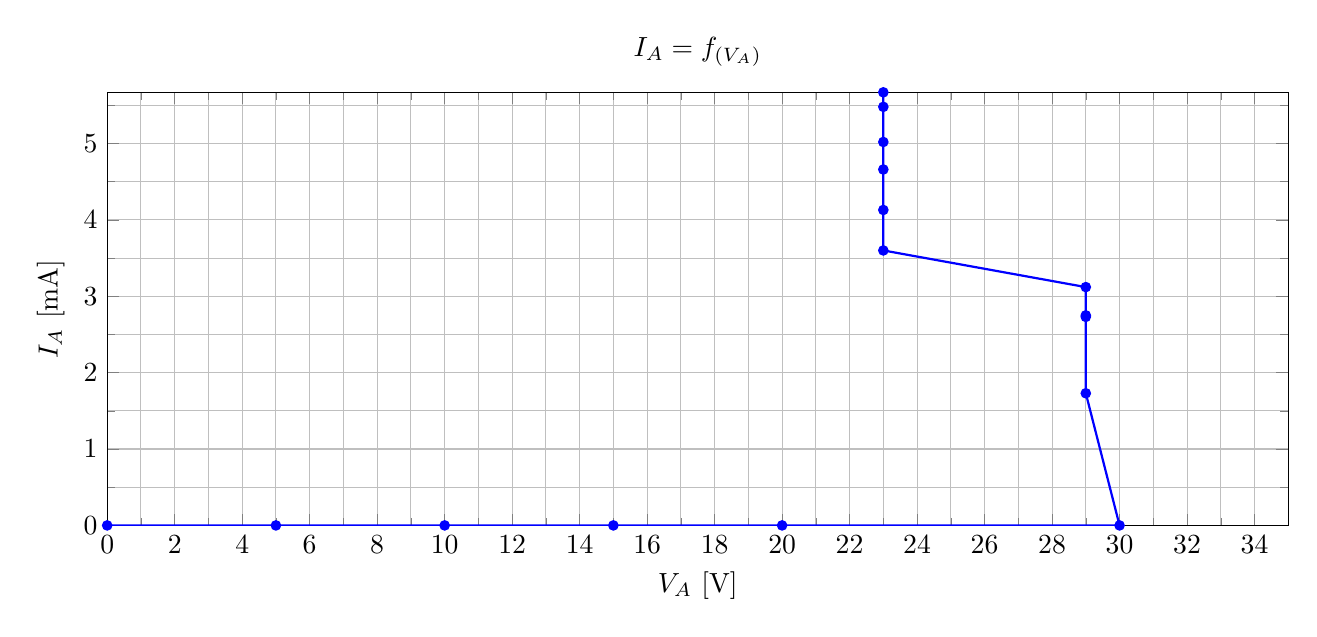
\begin{tikzpicture}
        \begin{axis}[
          width=15cm,
          height=5.5cm,
          xlabel={$V_{A}$ [V]},
          ylabel={$I_{A}$ [mA]},
          grid=both,
          minor tick num=1,
          scale only axis,
          enlargelimits=false,
            title={$I_{A} = f_{(V_A)}$},
          extra x tick style={
            grid style={red, thick, dashed},
            tick style={red},
            tick label style={red}
           },
          scaled ticks=false,
          restrict x to domain=0:35,
          xmin=0, xmax=35
        ]
        \addplot[
          color=blue,
          mark=*,
          mark size=1.5pt,
          thick
        ] coordinates {
          (0,0)
          (5,0)
          (10,0)
          (15,0)
          (20,0)
          (30,0)
          (29,1.73)
          (29,2.73)
          (29,2.75)
          (29,3.12)
          (23,3.6)
          (23,4.13)
          (23,4.66)
          (23,5.02)
          (23,5.48)
          (23,5.67)
        };
        \end{axis}
      \end{tikzpicture}
      \caption{gráfica $I_A = f_{(V_A)}$ relevada en el laboratorio.}
      \label{graph:diac}
    \end{figure}

    Como puede ver en la figura \ref{graph:diac}, la curva relevada en el laboratorio tiene cierta semejanza a la
    teórica del DIAC. Se puede apreciar que al rededor de $V_A = 30V$ empieza a haber una circulación de corriente, por
    lo que podemos decir que el $V_{BR(F)}$ del DIAC seleccionado esta cerca de los 30V. A medida que continuamos
    subiendo el voltaje, la corriente también fue subiendo, con una disminución del voltaje $V_A$ entre los pines del
    DIAC. En particular, este DIAC tiene una $I_H$ considerablemente grande para el voltaje máximo de operación, por lo
    que la curva no presenta esa disminución prácticamente instantánea de $V_A$ tan característica de los tiristores
    cuando comienza a conducir corriente.
